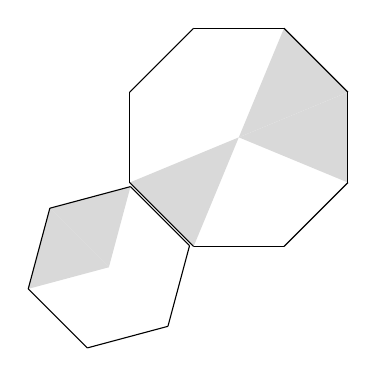
\begin{tikzpicture}[scale=0.75]
\def\radius{2}
\def\smallradius{1.414}
\foreach \angle [count=\i] in {180,225,...,495} {
\coordinate (A\i) at (\angle+22.5:\radius);
}
\foreach \i [remember=\i as \lasti (initially 1)] in {2} {
\fill[gray!30] (0,0) -- (A\i) -- (A\lasti) -- cycle;
}
\foreach \i [remember=\i as \lasti (initially 6)] in {5,4} {
\fill[gray!30] (0,0) -- (A\i) -- (A\lasti) -- cycle;
}
\foreach \i [remember=\i as \lasti (initially 8)] in {1,...,8} {
\draw (A\lasti) -- (A\i);
}
\begin{scope}[shift={(-2.2,-2.2)}]
\foreach \angle [count=\i] in {180,240,...,480} {
\coordinate (B\i) at (\angle+15:\smallradius);
}
\foreach \i [remember=\i as \lasti (initially 5)] in {6,1} {
\fill[gray!30] (0,0) -- (B\i) -- (B\lasti) -- cycle;
}
\foreach \i [remember=\i as \lasti (initially 6)] in {1,...,6} {
\draw (B\lasti) -- (B\i);
}
\end{scope}
\end{tikzpicture}